\documentclass[../main.tex]{subfiles}
\begin{document}
\chapter{Countability}
\section{Countable Sets}
\subsection{Introduction to Countability}
We want to talk about the sizes of infinite sets, for example, $\N$ ``looks smaller'' than $\Z$ which seem ``a lot smaller'' than $\Q$, which seems ``even smaller than'' $\R$

\begin{definition}[Countable Set]
  \label{countableDef}
  We say that a set $X$ is \textit{countable} if $X$ is finite or there is a bijection $X \to \N$.

  This second case is often referred to as \textit{countably infinite}.
\end{definition}
That is, $X$ is countable if and only if we can enumerate the elements of $X$ using $\N$, i.e:
\[
  x_1, x_2, x_3, \ldots
\]
which terminates if $X$ is finite.
\begin{example}
  \begin{enumerate}
    \item Any finite set is countable.
    \item $\N$ is countable, or more specifically, countably infinite.
    \item $\Z$ is countable as we may list its elements as:
      \[
        0, 1, -1, 2, -2, \ldots
      \]
      That is, we can define a bijection $\N \to \Z$ given by $n \mapsto x_n$ where:
      \[
        x_n = \begin{cases}
        \frac{n}{2} & \text{ if $n$ even} \\
        -\frac{n - 1}{2} & \text{ if $n$ odd}
        \end{cases}
      \]
  \end{enumerate}
\end{example}
\begin{lemma}
  \label{countableSubset}
  Any subset of $\N$ is countable.
\end{lemma}
\begin{proof}
  If $S \subseteq \N$ is non empty, by the Well-Ordering Principle (\cref{WOP}), there is a least element $s_1 \in S$.

  If $S \setminus \{s_1\} \neq \emptyset$, again, there is a least element $s_2 \in S \setminus \{s_1\}$.

  If $S \setminus \{s_1, s_2\} \neq \emptyset$, ...

  If at some point this process terminates, then $S = \{s_1, s_2, \ldots, s_n\}$ is finite and therefore countable.

  Otherwise, if this process never terminates, then the map:
  \[
    g: \N \to S, n \mapsto s_n
  \]
  is well-defined, as, for every $n$ there will be a unique minimal element $s_n$.
  This map will be injective as when a least element appears, it is removed from the set so the same least element cannot occur twice.

  It is also surjective because, if $k \in S$, then $k \in \N$ so there are less than $k$ elements of $S$ less than $k$, so $k = s_n$ for some $n \leq k$.

  So we have a bijection between $S$ and $\N$, thus $S$ is countably infinite.
\end{proof}
\begin{theorem}
  \label{countabilityEquivalence}
  The following statements are equivalent:
  \begin{enumerate}
    \item $X$ is a countable set.
    \item There exists an injection from $X \to \N$.
    \item $X = \emptyset$ or there is a surjection $\N \to X$.
  \end{enumerate}
\end{theorem}
\begin{proof}\par
  (\textbf{i} $\implies$ \textbf{ii})
  \begin{indentenvironment}
    If $X$ is finite, then we can obviously find an injection into $\N$.
    Otherwise, if $X$ is in bijection with $\N$, then it certainly injects into $\N$.
  \end{indentenvironment}
  (\textbf{ii} $\implies$ \textbf{i})
  \begin{indentenvironment}
    If there is an injection $f: X \to \N$, then $f$ is a bijection between $X$ and $S = f(X)$.
    That is we can make $f$ a bijection by restricting the codomain to just the image of $X$.

    If $S$ is finite, then so is $X$ so $X$ is countable.

    Otherwise, if $S$ is infinite since $S \subseteq \N$ by \cref{countableSubset}, $S$ is countable.
    Therefore there is a bijection from $g: S \to \N$ and so
    \[
      X \xrightarrow{f} S= f(X) \xrightarrow{g} \N
    \]
    so $f \circ g$ is a bijection from $X \to \N$ and thus $X$ is countable.
  \end{indentenvironment}
  (\textbf{i} $\implies$ \textbf{iii})
  \begin{indentenvironment}
    If $X$ is finite, then either $X = \emptyset$ or there is a surjection from $\N \to X$
    (Note that we cannot have a surjection $\N \to \emptyset$ as each element of $\N$ must be mapped to something).

    Otherwise, if $X$ is infinite, then, since $X$ is countable, there is a bijection $\N \to X$ which must also be a surjection.
  \end{indentenvironment}
  (\textbf{iii} $\implies$ \textbf{ii})
  \begin{indentenvironment}
    If $X = \emptyset$, then any function $X \to \N$ is vacuously injective.

    Otherwise, suppose that $X \neq \emptyset$ and there is a surjection $f: \N \to X$.
    Consider an element $a \in X$.
    Since $f$ is surjective, the preimage of $a$ is a non-empty subset of $\N$.
    Therefore, by WOP (\cref{WOP}), it must have a least element.
    Define $g: X \to \N$ by $g(a) = \min f^{-1}(\{a\})$.
    By construction, $g$ is injective as $f$ is a well defined function.
  \end{indentenvironment}
  So we have: \textbf{ii} $\iff$ \textbf{i} $\implies$ \textbf{iii} $\implies$ \textbf{ii}, thus, all the statements are equivalent.
\end{proof}
\begin{corollary}
  \label{subsetOfCountableSet}
  Any subset of a countable set is countable.
\end{corollary}
\begin{proof}
  If $Y \subseteq X$ and $X$ is countable, then there is therefore an injection $X \to \N$.
  We can just restrict the domain to $Y \to \N$ which is still injective so $Y$ is countable.
\end{proof}
We may now view ``countable'' as saying that a set is ``at most as big as $\N$''.
\subsection{Unions and Products of Countable Sets}
\begin{theorem}
$\N \times \N$ is countable
\end{theorem}
We will give two proofs of this.
\begin{proof}[Diagonalisation]
  We can enumerate the elements of $\N \times \N$ by traversing them diagonally as follows:
  \begin{center}
  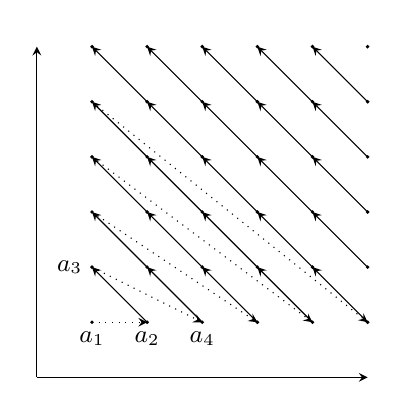
\begin{tikzpicture}[scale=0.7, >=stealth]
    \draw[->] (0, 0) -- (0, 6) node[above] {$\N$};
    \draw[->] (0, 0) -- (6, 0) node[right] {$\N$};

    \node[below] at (1, 1) {\small$a_1$};
    \node[below] at (2, 1) {\small$a_2$};
    \node[left] at (1, 2) {\small$a_3$};
    \node[below] at (3, 1) {\small$a_4$};

    \foreach \x in {1, 2, ..., 6} {
        \foreach \y in {1, 2, ..., 6} {
          \fill (\x, \y) circle (1pt);
          \ifnum \y < 6
            \ifnum \x = 1
              \draw[->, dotted] (\x, \y) -- (\x + \y, 1);
            \else
              \draw[->] (\x, \y) -- (\x - 1, \y + 1);
            \fi
          \fi
        }
    }
  \end{tikzpicture}
  \end{center}
  Define $a_1 = (1, 1)$ and $a_n$ inductively given $a_{n-1} = (p, q)$ by writing:
  \[
    a_n = \begin{cases}
    (p - 1, q + 1) & \text{ if } p \neq 1 \\
    (p + q, 1) & \text{ if } p = 1
    \end{cases}
  \]
  We can show by induction that this list includes every point $(x, y) \in \N \times \N$
\end{proof}
\begin{proof}[Injection]
  \label{ftaInjectiveProof}
  Define $f: \N \times \N \to \N$, $(x, y) \mapsto 2^{x}3^{y}$.
  Then $f$ is injective by the uniqueness of prime factorisations provided by the Fundamental Theorem of Arithmetic (\cref{uniquePrimeFactorisation}).
  So by \cref{countabilityEquivalence}, $\N \times \N$ is countable.
\end{proof}
\begin{corollary}
  $\Z \times \Z$ is countable.
\end{corollary}
\begin{proof}
  Since $\Z$ is countable, there is an injection $f: \Z \to \N$.
  We have just seen that $\N \times \N$ is countable so there is an injection $g: \N \times \N \to \N$.
  Hence, we have an injection:
  \[
    \Z \times \Z \xrightarrow{(f, f)} \N \times \N \xrightarrow{g} \N
  \]
  Thus $\Z \times \Z$ is countable by \cref{countabilityEquivalence}.
\end{proof}
\begin{remark}
  We can iterate this by induction to show that:
  \[
    \Z^{k} = \underbrace{\Z \times \cdots \times \Z}_{k \text{ copies}}
  \]
  is countable for any $k \in \N$.
\end{remark}
\begin{theorem}
  \label{countableUnion}
  A countable union of countable sets is countable.
\end{theorem}
\begin{proof}
  Since there is countably many of them, we may assume that our countable sets are indexed by $\N$.
  So given countable sets $A_1, A_2, \ldots$ (which may terminate) we wish to show that:
  \[
    \bigcup_{n \in \N} A_n \text{ is countable}
  \]
  For each $i \in \N$, since $A_i$ is countable, we may enumerate its elements as $a^{(i)}_{1}, a^{(i)}_{2}, a^{(i)}_{3}, \ldots$ (which may terminate)

  Define $f: \bigcup_{n \in \N} A_n \to \N$, $x \mapsto 2^{i}3^{j}$ where $x = a^{(i)}_{j}$ for the \textbf{least} $i$ such that $x \in A_i$ as $x$ could be in multiple sets, however by WOP, we can pick the least such $i$.
  This is an injection by the same argument as in \cref{ftaInjectiveProof}.

  Alternatively, the association of $x$ with a unique pair $(i, j)$ provides a injection $\bigcup A_n \to  \N \times \N$, which we know is countable.
\end{proof}
\begin{example}[Countability of $\Q$]
  We can define $\Q$ as:
  \[
    \Q = \bigcup_{n \in \N} \left\{\frac{m}{n}: m \in \Z\right\}
  \]
  This is a countable union of countable sets so $\Q$ is countable.
\end{example}
\begin{theorem}
  \label{ACountable}
  The set $\mathbb{A}$ of algebraic numbers is countable.
\end{theorem}
\begin{proof}
  It suffices to show that the set of all polynomials with integer coefficients is countable, as each polynomial has a finite number of roots (by \cref{fact2}), so $\mathbb{A}$ is a countable union of countable sets and is therefore countable by \cref{countableUnion}.

  In fact, it suffices to show that for each $d \in \N$, the set $P_d$ of all integer polynomials of degree $d$ is countable, as then the union of the sets of their roots is a countable union of countable sets.

  The map $P_d \to \Z^{d + 1}$,
  \[
    p(x) = a_d x^{d} + a_{d - 1}x^{d - 1} + \cdots + a_1 x + a_0 \mapsto (a_d, a_{d - 1}, \ldots, a_1, a_0)
  \]
  is an injection as each polynomial is uniquely defined by its coefficients.
  Since $\Z^{d + 1}$ is countable, $P_d$ is countable.
\end{proof}
\section{Uncountable Sets}
\begin{definition}[Uncountable]
  A set is \textit{uncountable} if it is not countable.
\end{definition}
\begin{theorem}
  $\R$ is uncountable.
  \label{RUncountable}
\end{theorem}
\begin{proof}[Cantor -- 1891]
  Suppose $\R$ is countable, we can then enumerate its elements as $r_1, r_2, r_3, \ldots$

  We can write each $r_n$ in decimal form:
  \begin{align*}
    r_1 &= n_1.d_{1 1}d_{1 2}d_{1 3}\ldots \\
    r_2 &= n_2.d_{2 1}d_{2 2}d_{2 3}\ldots \\
    r_3 &= n_3.d_{3 1}d_{3 2}d_{3 3}\ldots \\
        &\;\;\vdots
  \end{align*}
  Although we saw in \cref{decimalExpansionUniqueness} that decimal expansions are not unique, we can always just pick a specific decimal expansion to represent $r_i$.

  We then define the number $r = 0.d_1d_2d_3\ldots$ where:
  \[
    d_n = \begin{cases}
    1 & d_{n n} \neq 1 \\
    2 & d_{n n} = 1
    \end{cases}
  \]
  This $r$ has only one decimal expansion (as it does not terminate in all 0s or 9s) and is not in the enumerated list, as $\forall n \in \N$ $r \neq r_n$ as we have constructed it to disagree with $r_n$ on the $n$-th decimal digit.
  This contradicts the countability of $\R$.
\end{proof}
This proof strategy is known as a \textit{diagonal argument}.
\begin{remark}
  This proof did not use the integer part of each $r_i$ so we can conclude that the interval $(0, 1)$ is uncountable.
\end{remark}
\begin{corollary}
  There are uncountably many transcendental numbers.
\end{corollary}
\begin{proof}
  Suppose $\R \setminus \mathbb{A}$ is countable.
  We saw that $\mathbb{A}$ is countable in \cref{ACountable}, however, we can write $\R = (\R \setminus \mathbb{A}) \cup \mathbb{A}$ which is a countable union of countable sets, so by \cref{countableUnion}, $\R$ is countable which is a contradiction by the above.
\end{proof}
\begin{theorem}
  $\powerset{\N}$ is uncountable.
  \label{powerSetUncountable}
\end{theorem}
We will provide 2 proofs:
\begin{proof}[1 -- Diagonal Arugment]
  If $\powerset{\N}$ were countable, we would be able to enumerate its elements as $S_1, S_2, S_3, \ldots$

  Similarly to in \cref{RUncountable}, we wish to construct a set that disagrees with each of our sets on one element.
  If we define:
  \[
    S = \{n \in \N: n \notin S_n\}
  \]
  then $S$ is not on our list since $\forall n \in \N$, $S \neq S_n$ as, by construction, they must disagree on the element $n$.
  This contradicts the countability of $\powerset{\N}$.
\end{proof}
\begin{proof}[2 -- Injection]
  We wish to show that there is an injection from $(0, 1) \to \powerset{\N}$ so that if $\powerset{\N}$ were countable, we would have an injection $\powerset{\N} \to \N$ and thus an injection $(0, 1) \to \N$ which contradicts \cref{RUncountable}.

  We start by writing $x \in (0, 1)$ in binary:
  \[
    0.x_1x_2x_3\ldots
  \]
  with $x_i \in \{0, 1\}$.
  Since the binary representation of $x$ is not necessarily unique, we pick those not ending in an infinite string of 1s.

  We then define:
  \[
    f(x) = \{n \in \N: x_n = 1\}
  \]
  For example, $f(0.1110100000\ldots) = \{1, 2, 3, 5\}$.
  This is a well-defined injection as each subset of $\N$ uniquely defines such a binary expansion.
\end{proof}
\begin{remark}
  Note that we are not requiring $f$ to be surjective, as $\{n \in \N: n > 5\}$ cannot be the image of any $x$ as this it would need to end in an infinite string of $1$s.
\end{remark}
The first proof of this theorem can also be used to show the following:
\begin{theorem}
  For any set $X$, there does \textbf{not} exist a bijection between $X$ and $\powerset{X}$.
\end{theorem}
\begin{proof}
  Given any $f: X \to \powerset{X}$, we can show that it cannot be surjective.

  Indeed, let $S = \{x \in X: x \notin f(x)\}$.
  Certainly $S \in \powerset{X}$ and $S$ is not in the image of $f$, since for every $x \in X$, the sets $S$ and $f(x)$ differ in the element $x$.
  Thus $S \neq f(x)$ for all $x \in X$ so $f$ cannot be surjective and consequently cannot be  bijective.
\end{proof}
\begin{remark}[Remarks]
  \begin{enumerate}
    \item This is reminiscent of Russel's Paradox (\cref{russelsParadox}).
      However, our proof is valid as we used subset selection correctly by specifying a well defined set to select the elements from.
    \item In fact, it gives another proof that there is no universal set.

      Suppose we had a universal set $V$, then we would have $\powerset{V} \subseteq V$, in which case there would certainly be a surjection from $V$ onto $\powerset{V}$ as there is always a surjection from a set to one of its subsets.
      This is a contradiction by the above, thus, there is no universal set.
  \end{enumerate}
\end{remark}
\begin{proposition}
  If $\{A_i : i \in I\}$ is a family of open pairwise disjoint intervals of $\R$ indexed by the set $I$, then $I$ is countable.
  \label{intervalsExample}
\end{proposition}
We will provide 2 proofs:
\begin{proof}[1 -- Injection]
  We know that each interval $A_i$ contains a rational as, from \cref{rationalsDense}, $\Q$ is dense in $\R$.
  Since the intervals are disjoint, we can construct an injection from $I \to \Q$ by picking a rational from each interval.
  We know that $\Q$ is countable, so we now must have an injection $I \to \N$.
  Hence $I$ is countable.
\end{proof}
\begin{proof}[2 -- Union of Countable Sets]
  The set $S_1 = \{i \in I: A_i \text{ has length} \geq 1\}$ is countable as we can pick an integer from each $A_i$ with length $\geq 1$ and, since they are disjoint, use this to construct an injection into $\Z$.

  Similarly, the set $S_2 = \{i \in I: A_i \text{ has length}\geq 1/2\}$ is countable as it injects into the set of half integers which is countable by \cref{subsetOfCountableSet} as it is a subset of $\Q$.

  More generally, for each $n \in \N$, the set $S_n = \left\{i \in I : A_i \text{ has length} \geq \frac{1}{n}\right\}$ is countable as it injects into $\Z/n$.

  By \cref{archimedesCorollary}, for any length $\ell_n \in \R$ of $A_n$, we can find some $n \in \N$ such that $\frac{1}{n} < \ell_n$.
  This means that if we continue this construction for all $n \in \N$, every element of $I$ will be in at least one of these sets.
  We can then express $I$ as:
  \[
    I = \bigcup_{n = 1}^{\infty} S_n
  \]
  Thus, $I$ is countable by \cref{countableUnion} as it is a countable union of countable sets.
\end{proof}
\begin{remark}[Summary]\par
To show that a set $X$ is \textbf{countable}, we can:
\begin{enumerate}
  \item List/enumerate its elements -- \cref{countableDef}
  \item Construct an injection into $\N$ or another countable set -- \cref{countabilityEquivalence}
  \item Show it is a countable union of countable sets -- \cref{countableUnion}
  \item If the set is in or ``near'' $\R$, consider $\Q$ -- \cref{intervalsExample}
\end{enumerate}
To show that a set $X$ is \textbf{uncountable}, we can:
\begin{enumerate}
  \item Use a diagonal argument -- Assume countable and then show that we can construct an element that differs from every other element -- See \cref{RUncountable}
  \item Inject an uncountable set (e.g. $(0, 1)$ or  $\powerset{\N}$) into $X$ -- Cannot have an injection from $X$ into $\N$ otherwise we have a contradiction -- See \cref{powerSetUncountable}
\end{enumerate}
\end{remark}
\section{Functions and Sizes of Sets}
We have the following intuition about functions of different types between sets:
\begin{center}
\begin{tabular}{c|c}
Statement & Intuition \\
\hline
$A$ bijects with $B$ & $A$ and $B$ are of the same size \\
$A$ injects into $B$ & $A$ is at most as big as $B$ \\
$A$ surjects onto $B$ & $A$ is at least as big as $B$
\end{tabular}
\end{center}
For these interpretations to make sense, we need to check that ``$A$ is at most as big as $B$'' if and only if ``$B$ is at least as big as $A$'' so that our intuition about inequalities still holds even with sets.
This is confirmed by the following lemma:
\begin{lemma}
  Given non-empty sets $A$ and $B$, there exists an injection $f: A \to B$ if and only if there exists a surjection $g: B \to A$.
\end{lemma}
\begin{proof}
  \begin{proofdirection}{Suppose we have an injection $f: A \to B$}
    Fix some $a_0 \in A$.
    We wish construct a surjection $g: B \to A$.

    Define $g: B \to A$ by:
    \[
      b \mapsto \begin{cases}
      \text{unique $a \in A$ s.t. $f(a) = b$} &  \text{ if such an $a$ exists} \\
      a_0 & \text{ otherwise}
     \end{cases}
    \]
    The first case of this map satisfies the criterion for surjectivity, however we need to send elements of $B$ that were not mapped to by $f$ from $A$ so that $g$ is a well-defined function.
  \end{proofdirection}
  \begin{proofdirection}{Suppose we have a surjection $g: B \to A$}
    Define $f: A \to B$ by:
    \[
      a \mapsto \text{some $b \in B$ s.t. $g(b) = a$}
    \]
    Then $f$ is injective as $g$ is a well-defined map.
  \end{proofdirection}
\end{proof}
Another intuition from inequalities we wan to confirm is that that, if ``$A$ is at most as big as $B$'' and ``$B$ is at most as big as $A$'', then
``$A$ and $B$ have the same size''.
\begin{theorem}[Schr\"oder Bernstein Theorem]
  \label{schroderBerstein}
  If $f: A \to B$ and $g: B \to A$ are injections, then there exists a bijection $h: A \to B$.
\end{theorem}
\begin{proof}
  For some point $a \in A$, write $g^{-1}(a)$ for the unique $b \in B$ (if it exists) such that $g(b) = a$.

  Similarly, for $b \in B$, write $f^{-1}(b)$ for the unique $a \in A$ (if it exists) such that $f(a) = b$.

  We call:
  \[
    g^{-1}(a),\ f^{-1}(g^{-1}(a)),\ g^{-1}(f^{-1}(g^{-1}(a))),\ \ldots
  \]
  the \textit{ancestor sequence} of the point $a \in A$.
  This terminates if the preimage does not exist at at some step.
  We define the ancestor sequence for $b \in B$ similarly.

  Let:
  \begin{align*}
    A_0 &= \{a \in A : \text{ ancestor sequence of $a$ stops after an even number of steps}\} \\
    A_1 &= \{a \in A : \text{ ancestor sequence of $a$ stops after an odd number of steps}\} \\
    A_{\infty} &= \{a \in A : \text{ ancestor sequence of $a$ does not terminate}\}
  \end{align*}
  and define $B_0, B_1, B_{\infty}$ similarly.
  Intuitively, $A_0$ is the set of elements of $A$ such that their ancestor sequence ends in $A$ and there are similar intuitions for $A_1, B_0$ and $B_1$.
  Since each element is in exactly one of these three sets, they partition $A$ and $B$ respectively.

  If we restrict $f: A_0 \to B_1$, it is injective by hypothesis and we can show that it is surjective.
  Every $b \in B_1$ terminates in an odd number of steps so has at least one ancestor.
  Therefore for some $a \in A_0$ we have $f(a) = b$ (If we take $a = f^{-1}(b)$ we see that this terminates after an even number of steps as the ancestor sequence for $b$ has an odd number of steps, so $a \in A_0$).
  Thus we have a bijection between $A_0$ and $B_1$ given by $f$.

  By symmetry, $g$ bijects $B_0$ with $A_1$.

  Finally, by a similar argument, both $f$ and $g$ provide a bijection between $A_{\infty}$ and $B_{\infty}$ as these are the points whose ancestor sequence never terminates.

  Then the function $h: A \to B$ defined by:
  \[
    a \mapsto \begin{cases}
    f(a) & \text{ if }a \in A_0 \cup A_{\infty} \\
    g^{-1}(a) & \text{ if }a \in A_1 \\
    \end{cases}
  \]
  is a bijection by construction.
\end{proof}
\begin{example}
  Is there a bijection from $[0, 1]$ to $[0, 1] \cup [2, 3]$?

  Observe that we have an injection $f: [0, 1] \to [0, 1] \cup [2, 3]$, $x \mapsto x$ and an injection $g: [0, 1] \cup [2, 3] \to [0, 1]$, $x \mapsto x/3$.
  So by \cref{schroderBerstein}, there is a bijection between them.
\end{example}
\begin{remark}[Remarks]
  \begin{enumerate}
    \item It would be nice to be able to say that for any sets $A$ and $B$, either $A$ injects into $B$, or $B$ injects into $A$.

      This is in fact true but is more difficult to prove, see Logic and Set Theory.
    \item The \textit{Continuum Hypothesis} states that there does not exist a set whose size lies between $\N$ and $\R$.
      That is, any subset of $\R$ is either finite, countably infinite, or uncountable (in bijection with $\R$).
      It has been shown that in ZFC (\textit{Zermelo–Fraenkel set theory}), it is impossible to prove or disprove the continuum hypothesis.
  \end{enumerate}
\end{remark}
\end{document}
